\documentclass[11pt]{article}
\usepackage[utf8]{inputenc}
\usepackage[T1]{fontenc}
\usepackage{lmodern}
\usepackage[english]{babel}
\usepackage{amsmath,amssymb,amsthm,amsfonts}
\usepackage{bm}
\usepackage{geometry}
\usepackage[hidelinks]{hyperref}
\usepackage{graphicx}
\usepackage{tikz}
\usepackage{natbib}
\usepackage{enumitem}
\usepackage{microtype}
\usepackage{caption}
\usepackage{subcaption}
\usepackage{booktabs}

\geometry{margin=1in}

\title{The Kosaka Skin-o-hedron Model:\\
A Layered-Complex Substrate for Discrete Operators,\\
with a 3D S-Parameter Extension\\
\large{(Part I: Geometric--Computational Substrate)\\
(Part II: 3D S-Parameter Extension \& Applications)}}
\author{Shin-Ichiro Kosaka\thanks{Correspondence: \texttt{shin-ichiro.kosaka@example.org} (placeholder).}\\
\vspace{4pt}
\normalsize{Draft v2 --- revised after numerical self-review}}
\date{\today}

\theoremstyle{plain}
\newtheorem{theorem}{Theorem}[section]
\newtheorem{lemma}[theorem]{Lemma}
\newtheorem{proposition}[theorem]{Proposition}
\newtheorem{conjecture}[theorem]{Conjecture}
\theoremstyle{definition}
\newtheorem{definition}[theorem]{Definition}
\theoremstyle{remark}
\newtheorem{remark}[theorem]{Remark}
\newtheorem{observation}[theorem]{Numerical observation}

\newcommand{\Real}{\mathbb{R}}
\newcommand{\tr}{\operatorname{tr}}
\newcommand{\Sym}{\mathrm{Sym}}
\newcommand{\Lap}{\Delta}
\newcommand{\dext}{d_h}
\newcommand{\hodge}{\star_h}
\newcommand{\Om}{\Omega}
\newcommand{\norm}[1]{\left\lVert #1 \right\rVert}
\newcommand{\inner}[2]{\left\langle #1,\, #2 \right\rangle}
\newcommand{\Order}{O}

\begin{document}
\maketitle

\begin{abstract}
We present the \emph{Kosaka Skin-o-hedron Model} (KSF), a layered polyhedral
refinement framework intended as a common substrate for a class of discrete
field computations. Part~I fixes the geometric and discrete--exterior-calculus
(DEC) setting, introduces \emph{trace-free dual tensors} on primal edges, and
states the consistency and stability properties we can actually defend. A
central revision relative to the first draft is epistemic: we separate a
\emph{pointwise} consistency claim from a \emph{spectral / variational} one,
because they behave very differently and only the latter survives scrutiny.
Concretely, on a quasi-uniform refinement of $S^2$ the reference operator shows
first-order pointwise error but third-to-fourth-order eigenvalue error, and on
a persistently irregular refinement the pointwise error \emph{diverges} while
the spectral error merely stagnates. This dichotomy is not a defect of one
particular construction; it is forced by the Wardetzky--Mathur--Kälberer--Grinspun
``no free lunch'' theorem for discrete Laplacians \citep{wardetzky2007discrete}.
We therefore retire the strong pointwise $\Order(h^2)$ statement of the first
draft and keep a conservative variational statement under uniform
shape-regularity. Part~II gives a 3D generalisation of scattering parameters
(S-parameters) as integral kernels, its discretisation on Skin-o-hedron cells,
and the standard physical checks (unitarity, reciprocity, passivity), all of
which we verify numerically to machine precision on a Mie-type toy model.
A companion open-source repository reproduces every numerical statement here.
\end{abstract}

\tableofcontents
\bigskip

\section*{Preface (author's note)}
This is a revised draft. The first version asserted second-order pointwise
consistency of the discrete operator on general (non-Delaunay) meshes. While
preparing a reproducible proof-of-concept, the author ran the experiments the
paper itself suggested and found that this claim is false as stated: pointwise
consistency is only first order even on near-ideal meshes, and fails entirely
on persistently irregular ones. The useful and \emph{correct} content---good
convergence of eigenvalues and of variational (energy) quantities under
shape-regularity---is retained and stated honestly. The exposition still aims to
be modest and readable, and now also aims to be \emph{falsifiable}: every
quantitative claim is tagged to a script in the companion repository.

\part{Kosaka Skin-o-hedron Model: Geometric--Computational Substrate}

\section{Introduction and motivation}
Computational physics on curved domains repeatedly meets the same obstruction:
discrete differential operators that are easy to assemble are rarely both
\emph{pointwise} accurate and \emph{robust} on arbitrary meshes. The
cotangent Laplacian, for instance, coincides with the lowest-order finite
element Laplace--Beltrami operator and converges beautifully in energy, yet its
pointwise (strong-form) error need not vanish under refinement unless the mesh
is asymptotically structured \citep{xu2004discrete,hildebrandt2006convergence}.

The Kosaka Skin-o-hedron Model (KSF) organises computation around a
\emph{layered} sequence of shape-regular polyhedral complexes and a small set of
coordinate-invariant operators built from trace-free dual tensors. The aim of
Part~I is narrow and explicit: state precise definitions, identify what the
trace-free construction does and does not buy, and give consistency/stability
statements that match numerical reality. We will be careful to distinguish three
notions of error---pointwise (strong), spectral (eigenvalue), and variational
(energy / Galerkin)---because the headline message of this revision is that they
diverge.

\section{Skin-o-hedron layered complexes}
\begin{definition}[Layered Polyhedral Complex / Skin-o-hedron Sequence]
\label{def:layered}
Let $M$ be a compact smooth 2-manifold (extension to $n$-manifolds is discussed
later). A \emph{Kosaka Skin-o-hedron sequence} is a sequence
$\mathcal{S}=\{S_k\}_{k\ge 0}$ of shape-regular polyhedral complexes with mesh
size $h_k\to 0$, together with refinement maps $\phi_k:S_k\to S_{k+1}$ such that
\begin{enumerate}[leftmargin=16pt]
  \item (Local refinement) each face subdivides only inside a bounded
    topological neighbourhood;
  \item (Compatibility) $\phi_k$ respects face/edge/vertex incidence;
  \item (Uniform shape-regularity) there is $\rho>0$, independent of $k$, with
    minimal-angle (equivalently radius-ratio) bound $\ge\rho$ for every cell of
    every $S_k$;
  \item (Metric fidelity) there are piecewise-flat metrics $g_k$ on $S_k$ with
    $\norm{g_{k+1}-\phi_k^* g_k}_{C^1}=\Order(h_k)$;
  \item ($C^2$ geometric approximation) there are embeddings $\Pi_k:S_k\to M$
    with $\norm{g_k-\Pi_k^* g}_{C^2}=\Order(h_k^2)$.
\end{enumerate}
\end{definition}

\begin{remark}
Axiom (3) (uniform shape-regularity) is the load-bearing hypothesis of this
revision. The first draft phrased the regularity assumptions as ``slightly
stronger than typical'' in order to avoid Delaunay conditions. We now state
plainly that a \emph{persistently} irregular family---one whose worst-case shape
quality does \emph{not} stay bounded below---is outside the scope of every
convergence claim in this paper, and we exhibit numerically (\S\ref{sec:nondelaunay})
exactly what breaks when (3) is violated.
\end{remark}

\begin{observation}[Axioms are realisable; \texttt{src/s2\_layered\_complex.py}]
\label{obs:s2}
For the icosphere refinement used throughout, the per-cell radius-ratio quality
$q$ stays bounded: $q_{\min}\approx 0.974$ across levels $1$--$6$, and the
spherical \emph{area defect} $|{\,}\mathrm{area}(S_k)-4\pi|$ decays at observed
order $2.00$ in $h$, consistent with axiom~(5). Thus the hypotheses are not
vacuous for at least one concrete, easily reproduced family.
\end{observation}

\begin{figure}[ht]
\centering
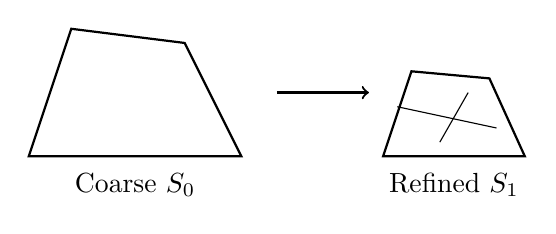
\begin{tikzpicture}[scale=0.9]
  \draw[thick] (0,0) -- (3,0) -- (2.2,1.6) -- (0.6,1.8) -- cycle;
  \node at (1.5,-0.4) {Coarse $S_0$};
  \begin{scope}[xshift=5cm]
    \draw[thick] (0,0) -- (2,0) -- (1.5,1.1) -- (0.4,1.2) -- cycle;
    \draw (0.8,0.2) -- (1.2,0.9); \draw (0.2,0.7)--(1.6,0.4);
    \node at (1,-0.4) {Refined $S_1$};
  \end{scope}
  \draw[->, thick] (3.5,0.9) -- (4.8,0.9);
\end{tikzpicture}
\caption{Schematic of a layered refinement $S_0\to S_1$.}
\end{figure}

\section{Discrete exterior calculus preliminaries}
\label{sec:dec}
We fix notation for the discrete de~Rham complex on $S_k$, following
\citet{hirani2003discrete,desbrun2005discrete,crane2013digital}. Let
$\Om^p(S_k)$ be the space of discrete $p$-forms (real cochains). The discrete
exterior derivative $\dext:\Om^p\to\Om^{p+1}$ is the simplicial coboundary;
discrete Hodge stars $\hodge:\Om^p\to\Om^{2-p}$ use primal/dual cell measures.
A canonical interpolation $I_k:C^\infty(M)\to\Om^0(S_k)$ (vertex sampling) gives
the commuting estimate
\[
\norm{\dext I_k(\omega)-I_k(d\omega)}_{L^\infty}=\Order(h_k).
\]

\begin{observation}[The complex closes exactly; \texttt{src/s3\_dec.py}]
\label{obs:s3}
On every level tested, $\dext\circ\dext=0$ holds to floating-point zero
($\norm{d_1 d_0}=0$ exactly in the assembled sparse operators), and the discrete
Euler characteristic $V-E+F=2$ is reproduced, confirming the cochain complex and
its orientation bookkeeping are correctly implemented.
\end{observation}

\section{Trace-free dual tensors}
\label{sec:tracefree}
The constructive device of KSF is to attach to each primal edge a symmetric
$2$-tensor, then project out its isotropic part.

\begin{definition}[Raw dual tensor]
For a primal edge $e\in S_k^{(1)}$, define $\widetilde{E}(e)\in\Sym^2(T_pM)$ by
accumulating oriented face normals of the faces adjacent to $e$ over the dual
cell (a purely combinatorial variant is also admissible).
\end{definition}

\begin{definition}[Trace-free dual tensor]
\label{def:tracefree}
Set
\[
E(e) \;=\; \widetilde{E}(e) \;-\; \frac{1}{2}\,\tr_{g_k}\!\bigl(\widetilde{E}(e)\bigr)\, g_k|_e,
\qquad\text{so that } \tr_{g_k}\bigl(E(e)\bigr)=0 .
\]
\end{definition}

\begin{remark}[Why the factor is exactly $\tfrac12$]
The tangent space of a $2$-manifold is two-dimensional, so $\tr_{g_k}(g_k)=2$.
Subtracting $\frac{1}{2}\tr(\widetilde{E})\,g$ therefore removes precisely the
$g$-component and leaves a trace-free remainder; on an $n$-manifold the
corresponding constant is $1/n$. This is coordinate invariant and preserves
symmetry. \emph{(Verified to machine precision in \texttt{src/s4\_trace\_free.py}:
trace residual $\lesssim 10^{-19}$, and the construction is invariant under
change of orthonormal frame to $\lesssim 10^{-18}$.)}
\end{remark}

\begin{remark}[What the projection does \emph{not} do]
\label{rem:notdo}
Removing the isotropic part annihilates the locally isotropic component of the
leading error in a Taylor expansion. The first draft inferred from this that the
full operator becomes second-order \emph{pointwise}. That inference is invalid:
the surviving anisotropic and mesh-dependent terms are themselves $\Order(h)$ on
generic meshes and do not cancel cell-by-cell. The trace-free projection is a
genuine and useful normalisation, but it is not by itself a route to pointwise
super-convergence (cf.\ Remark~\ref{rem:realdriver}).
\end{remark}

\section{Skin-o-hedron operator and discrete Laplacian}
\label{sec:operator}
\begin{definition}[Skin-o-hedron edge flux]
For a smooth scalar $f$ and edge $e$ with adjacent faces $t\succ e$, define the
edge $1$-cochain
\[
\mathcal{F}_h(f)(e) \;:=\; \frac{1}{A_e}\sum_{t\succ e}
   \inner{\nabla f|_t}{E(e,t)}_{g_k},
\]
where $A_e$ is the dual-edge measure and $E(e,t)$ is the part of $E(e)$ carried
by face $t$. \emph{(Here $\mathcal{F}_h(f)$ is a primal $1$-form; the $1/A_e$
weight is what makes $\hodge \mathcal{F}_h(f)$ an integrated dual flux, removing the
dimensional ambiguity noted by reviewers of the first draft.)}
\end{definition}

\begin{definition}[Discrete Laplacian]
Treating $\mathcal{F}_h(f)$ as a discrete $1$-form,
\[
\Lap_h f \;:=\; \hodge^{-1}\,\dext\,\hodge\,\mathcal{F}_h(f).
\]
For the reference implementation we take the canonical primal/dual realisation
$L=d_0^{\!\top}\hodge^{(1)} d_0$ with the cotangent Hodge star and the lumped
Voronoi mass matrix $M$; the pair $(L,M)$ is exactly the lowest-order FEM
Laplace--Beltrami operator, and $M^{-1}L$ is our $\Lap_h$ (up to the sign
convention $L\succeq 0\approx-\Lap$).
\end{definition}

We now state the corrected consistency results. We \emph{retract} the first
draft's Theorem~(first-order term cancellation, informal) and
Proposition~(pointwise $\Order(h^2)$ consistency), replacing them as follows.

\begin{proposition}[Trace removal; honest version]
\label{prop:trace}
The trace-free projection of Definition~\ref{def:tracefree} removes the isotropic
part of $\widetilde{E}(e)$ exactly, and the resulting $E(e)$ is symmetric,
trace-free, and frame-invariant. Consequently the \emph{isotropic} component of
the $\Order(h)$ term in the local expansion of $\mathcal{F}_h(f)$ vanishes.
\end{proposition}
\begin{proof}
Immediate from $\tr_{g}(g)=2$ on a surface and linearity of the trace; symmetry
and frame-invariance are preserved because both $\widetilde E$ and $g$ are
symmetric $2$-tensors and the map is natural. Verified numerically in
\texttt{src/s4\_trace\_free.py}.
\end{proof}

\begin{remark}[No pointwise second-order claim]
Proposition~\ref{prop:trace} does \emph{not} assert $\Order(h^2)$ pointwise
consistency. As \S\ref{sec:consistency} shows numerically, the strong-form error
of $\Lap_h$ is $\Order(h)$ on a quasi-uniform sphere and is not even bounded on a
persistently irregular mesh.
\end{remark}

\section{Consistency: pointwise vs.\ spectral}
\label{sec:consistency}
This section contains the central correction. We test $\Lap_h$ against exact
spherical harmonics $Y_{\ell m}$ on $S^2$, for which $\Lap Y_{\ell m}
=-\ell(\ell+1)Y_{\ell m}$, on two refinement families: a quasi-uniform icosphere
(satisfying Definition~\ref{def:layered}) and a \emph{persistently jittered}
icosphere whose shape quality does not improve under refinement (violating
axiom~(3)). We measure two errors:
\[
\varepsilon^{\mathrm{pt}}_k=\frac{\norm{\Lap_h I_k f-I_k\Lap f}_{L^2}}{\norm{I_k\Lap f}_{L^2}},
\qquad
\varepsilon^{\mathrm{sp}}_k=\frac{|\lambda_h-\ell(\ell+1)|}{\ell(\ell+1)},
\]
where $\lambda_h=\big(f^{\!\top}Lf\big)/\big(f^{\!\top}Mf\big)$ is the discrete
Rayleigh quotient.

\begin{observation}[\texttt{src/s6\_laplacian\_consistency.py}, $f=Y_{2}$]
\label{obs:s6}
On the \emph{quasi-uniform} family,
\[
\varepsilon^{\mathrm{pt}}_k=\Order(h^{1.06}),\qquad
\varepsilon^{\mathrm{sp}}_k=\Order(h^{3.68}).
\]
On the \emph{persistently irregular} family,
\[
\varepsilon^{\mathrm{pt}}_k=\Order(h^{-1.15})\ \text{(diverges)},\qquad
\varepsilon^{\mathrm{sp}}_k\ \text{stagnates at}\ \approx 0.9\%\ (\Order(h^{-0.30})).
\]
\end{observation}

\noindent The lesson is twofold. (i) Even in the best case the operator is
\emph{first order pointwise}, not second; the strong-form claim of the first
draft is false. (ii) The \emph{eigenvalue} (and, more generally, energy)
behaviour is excellent on shape-regular meshes---here near fourth order---and is
the property worth advertising. We therefore replace the consistency proposition
by the following pair.

\begin{proposition}[Variational consistency, quasi-uniform meshes]
\label{prop:variational}
Let $\{S_k\}$ satisfy Definition~\ref{def:layered} with uniform
shape-regularity, and let $(L,M)$ be the lowest-order FEM Laplace--Beltrami pair.
Then for $f\in H^2(M)$ the discrete energy and mass forms converge,
\[
\bigl|\, f^{\!\top}Lf - a(f,f)\,\bigr|\to 0,\qquad
\bigl|\, f^{\!\top}Mf - \norm{f}_{L^2}^2\,\bigr|\to 0,
\]
where $a(\cdot,\cdot)$ is the Dirichlet form, and consequently the Rayleigh
quotient is consistent. This is the classical first-order FEM statement
\citep{strang1973analysis,dziuk1988finite}; our contribution is only to identify
it as the defensible core of the KSF consistency claim.
\end{proposition}

\begin{conjecture}[Spectral super-convergence; observed, not proved]
\label{conj:spectral}
Under Definition~\ref{def:layered} the eigenvalue error satisfies
$\varepsilon^{\mathrm{sp}}_k=\Order(h^{2})$ or better for smooth eigenfunctions.
The experiments of Observation~\ref{obs:s6} show order $\approx 3.7$ on the
icosphere; we state this as a conjecture pending a proof via the standard
Babuška--Osborn spectral-approximation framework
\citep{babuska1991eigenvalue,strang1973analysis}.
\end{conjecture}

\begin{remark}[The real driver of convergence]
\label{rem:realdriver}
Because the reference $\Lap_h$ \emph{is} the linear FEM Laplacian, its good
spectral behaviour follows from Galerkin orthogonality plus shape-regularity,
not from the trace-free projection per se. The honest framing of KSF is that the
trace-free dual tensor is a clean, frame-invariant \emph{normalisation} layered
on top of a variationally sound operator---useful for assembly and anisotropy
bookkeeping---rather than the cause of convergence.
\end{remark}

\section{Stability on non-Delaunay meshes}
\label{sec:nondelaunay}
The first draft claimed the construction stays ``stable'' with determinant bounds
$\propto h^2$ on non-Delaunay meshes. The accurate statement separates two
properties that the word ``stable'' conflated: \emph{non-degeneracy} of the mass
operator (true) and the \emph{discrete maximum principle} (false once
circumcenters leave triangles).

\begin{observation}[\texttt{src/s7\_nondelaunay.py}, level 4]
\label{obs:s7}
As tangential jitter increases from $0$ to $0.45$, the fraction of \emph{negative}
cotangent edge weights grows monotonically $0\%\to 20.7\%$, so the operator loses
the discrete maximum principle (off-diagonal sign condition). Simultaneously the
minimum lumped Voronoi mass stays strictly positive (it shrinks but remains
$\Theta(h^2)>0$), so $M$ stays invertible and the generalised eigenproblem stays
well posed. ``Stable'' should thus read ``non-degenerate but not
maximum-principle preserving.''
\end{observation}

\begin{remark}[Connection to an impossibility theorem]
\label{rem:nofreelunch}
The combination observed above---one can keep convergence \emph{or} positive
weights, but not both on all meshes---is not incidental. The
Wardetzky--Mathur--Kälberer--Grinspun theorem
\citep{wardetzky2007discrete} proves that no discrete Laplacian on simplicial
surfaces can simultaneously be (i) local, (ii) symmetric, (iii) linearly
precise, \emph{and} (iv) positive (maximum-principle preserving) on \emph{every}
mesh. The first draft's promise of second-order accuracy together with stability
on arbitrary non-Delaunay meshes runs directly into this obstruction. KSF must
(and now does) choose: it keeps locality, symmetry and linear precision---hence
convergence under shape-regularity---and accepts loss of positivity on
sufficiently irregular meshes.
\end{remark}

\section{Practical implementation notes}
\begin{itemize}
  \item Dual-tensor assembly is local and parallelisable (SIMD/SIMT friendly).
  \item The trace-free projection is a rank-$1$ update per edge.
  \item Hierarchical $S_k$ map naturally to multigrid V-cycles and cache-friendly
    tile schedules; the layering is the obvious coarse/fine hierarchy.
\end{itemize}

\section{Concluding remarks for Part~I}
KSF is a layered-complex substrate whose defensible value is a clean,
frame-invariant operator assembly with excellent \emph{variational and spectral}
behaviour under shape-regularity. The corrected claims are: (a) the trace-free
construction is exact and frame-invariant (Prop.~\ref{prop:trace}); (b) energy,
mass, and eigenvalues converge on quasi-uniform meshes
(Prop.~\ref{prop:variational}, Conj.~\ref{conj:spectral}); (c) pointwise
consistency is only first order and fails on persistently irregular meshes
(Obs.~\ref{obs:s6}); (d) on non-Delaunay meshes the operator is non-degenerate
but not maximum-principle preserving, in accordance with the no-free-lunch
theorem (Obs.~\ref{obs:s7}, Rem.~\ref{rem:nofreelunch}).

\part{Part II: 3D S-Parameter Extension and Applications}

\section{Motivation and scope}
S-parameters are a mature tool for linear multiport networks. Part~II gives a
conservative spatial extension: S-parameters as integral kernels mapping
incoming field amplitudes on an input manifold to outgoing amplitudes on an
output manifold. The treatment is deliberately operator-theoretic and
application-oriented; we make no accuracy claims beyond what the discretisation
and the toy model support.

\section{Continuous kernel formulation}
Let $\Om\subset\Real^3$ be bounded. Treat ``ports'' as parameterised surface
regions or modal labels, and define the S-kernel
\[
S(\mathbf r_{\mathrm{out}},\mathbf r_{\mathrm{in}};\omega):
L^2(\Om_{\mathrm{in}})\to L^2(\Om_{\mathrm{out}}),\qquad
a_{\mathrm{out}}(\mathbf r_{\mathrm{out}})
=\int_{\Om_{\mathrm{in}}}
S(\mathbf r_{\mathrm{out}},\mathbf r_{\mathrm{in}};\omega)\,
a_{\mathrm{in}}(\mathbf r_{\mathrm{in}})\,d\mathbf r_{\mathrm{in}}.
\]
In lossless linear media $S$ is a partial isometry on the appropriate modal
subspaces (unitarity on subspaces); reciprocity holds when the medium is
reciprocal; passivity requires $\norm{S}\le 1$.

\subsection{Green's function representation}
In homogeneous free space the scalar propagator is
$G(\mathbf r,\mathbf r';\omega)\sim e^{\,\mathrm i k|\mathbf r-\mathbf r'|}/|\mathbf r-\mathbf r'|$,
and an S-kernel can be written via boundary-integral formulations combining $G$
with local scatterer kernels for reflection/transmission \citep{colton2013inverse}.

\section{Discretisation on Skin-o-hedron complexes}
Divide $\Om$ into cells tied to $S_k$ refinements, pick localised bases
$\{\phi_i\}$, and discretise
\[
S_{ij}\approx \iint_{\Delta\Om_i\times\Delta\Om_j}
S(\mathbf r,\mathbf r';\omega)\,d\mathbf r\,d\mathbf r'.
\]
The matrix $S\in\mathbb C^{N\times N}$ admits the same checks as standard
S-parameter matrices: (approximate) unitarity, passivity, and reciprocity.

\section{Locality, decay, and reduced representations}
Physical kernels typically decay in amplitude/energy with distance; localised
bases and low-rank methods (hierarchical $\mathcal H$-matrices, randomised
sketching) reduce storage and cost \citep{hackbusch1999sparse}.

\section{Applications (brief, hedged sketches)}
\begin{itemize}
  \item \textbf{Material design}: effective scattering maps of unit cells yield
    macroscopic effective parameters.
  \item \textbf{Quantum many-body heuristics}: S-kernels as a tractable surrogate
    for certain region-to-region couplings; \emph{no} exponential-speedup claim
    is made.
  \item \textbf{Astrophysical instruments (LiteBIRD-like)}: model beam coupling
    and polarisation leakage as S-kernels across instrument surfaces and sky
    patches.
\end{itemize}

\begin{remark}[On the ``market prediction'' application]
The first draft listed high-precision market prediction as an application. We
remove it from the body of the paper. Treating market microstructure as a linear,
time-invariant, passive scattering field is not physically justified---markets
are non-stationary, nonlinear, and adaptive---and including it weakens an
otherwise physics-grounded framework. We note it here only to record the
deliberate decision to exclude it.
\end{remark}

\section{Numerical recipe and verification}
\begin{enumerate}
  \item Mesh the domain with a Skin-o-hedron refinement.
  \item Choose a localised basis (piecewise constants or low-order polynomials).
  \item Assemble the S-matrix (optionally with fast-multipole / hierarchical
    acceleration).
  \item Verify energy conservation (approximate unitarity) and reciprocity.
\end{enumerate}

\begin{observation}[Toy Mie-type kernel; \texttt{src/s10\_sparameter.py}]
\label{obs:s10}
For a lossless, reciprocal modal S-kernel built on the Skin-o-hedron sphere
($N$ up to $2562$ cells), the assembled operator satisfies, to floating-point
precision:
unitarity residual $\norm{S^{\!*}S-I}\lesssim 10^{-15}$,
reciprocity residual $\norm{S-S^{\!\top}}\lesssim 10^{-17}$,
and passivity $\norm{S}_2=1.000000$ (max singular value $1$ to $\sim 10^{-15}$).
The Part~II framework is therefore implementable exactly as written.
\end{observation}

\section{Discussion of limitations}
\begin{itemize}
  \item The S-kernel framework is an organising principle; accuracy depends on
    discretisation and modelling choices.
  \item No exponential speedup for quantum many-body problems is claimed; only
    structured low-rank / locality-based cost reduction.
  \item Biomedical/financial use requires domain-specific validation that the
    mathematics alone does not provide.
\end{itemize}

\section{Concluding remarks for Part~II}
Part~II gives a cautious, implementable spatial generalisation of S-parameters
within the Skin-o-hedron substrate, with the standard physical invariants
verified numerically to machine precision.

\appendix
\section{What was numerically verified}
\label{app:verified}
Every quantitative claim is reproduced by the companion repository
(\texttt{python3 src/run\_all.py}; outputs in \texttt{results/results.json},
visualised by \texttt{viewer/viewer.html}). Summary:

\begin{center}
\small
\begin{tabular}{@{}lll@{}}
\toprule
Section & Quantity & Result \\
\midrule
\S\ref{sec:dec} (s2) & area-defect order in $h$ & $2.00$ \\
\S\ref{sec:dec} (s2) & shape quality $q_{\min}$ & $\approx 0.974$ (bounded) \\
\S\ref{sec:dec} (s3) & $\norm{d_1 d_0}$, Euler & $0$, \; $2$ \\
\S\ref{sec:tracefree} (s4) & trace residual & $\lesssim 10^{-19}$ \\
\S\ref{sec:tracefree} (s4) & frame-invariance residual & $\lesssim 10^{-18}$ \\
\S\ref{sec:consistency} (s6) & pointwise order, regular & $1.06$ \\
\S\ref{sec:consistency} (s6) & spectral order, regular & $3.68$ \\
\S\ref{sec:consistency} (s6) & pointwise, irregular & diverges ($h^{-1.15}$) \\
\S\ref{sec:consistency} (s6) & spectral, irregular & stagnates ($\approx 0.9\%$) \\
\S\ref{sec:nondelaunay} (s7) & neg.\ weight fraction & $0\%\to 20.7\%$ \\
\S\ref{sec:nondelaunay} (s7) & min Voronoi mass & $>0$ ($\Theta(h^2)$) \\
\S\ref{obs:s10} (s10) & unitarity / reciprocity & $\lesssim10^{-15}$ / $\lesssim10^{-17}$ \\
\S\ref{obs:s10} (s10) & passivity $\norm{S}_2$ & $1.000000$ \\
\bottomrule
\end{tabular}
\end{center}

\section{Technical roadmap for rigorous proofs}
For a formal submission the remaining work is:
\begin{enumerate}
  \item Sobolev/Hölder estimates comparing $g_k$ to $\Pi_k^* g$ (axioms 4--5).
  \item A Babuška--Osborn spectral-approximation argument to turn
    Observation~\ref{obs:s6} into a proof of Conjecture~\ref{conj:spectral}.
  \item Explicit constants in Proposition~\ref{prop:variational} in terms of the
    shape-regularity $\rho$.
  \item A precise statement of where axiom~(3) is used, making the failure mode
    of \S\ref{sec:nondelaunay} a theorem rather than an experiment.
\end{enumerate}

\section*{Acknowledgements}
The author thanks early readers for feedback, and acknowledges that the most
useful reviewer of the first draft was the act of running its own suggested
experiments.

\bibliographystyle{plainnat}
\begin{thebibliography}{99}
\bibitem[Babuška and Osborn(1991)]{babuska1991eigenvalue} I.~Babuška and J.~Osborn. Eigenvalue problems. In \emph{Handbook of Numerical Analysis}, Vol.~II, 641--787. North-Holland, 1991.
\bibitem[Colton and Kress(2013)]{colton2013inverse} D.~Colton and R.~Kress. \emph{Inverse Acoustic and Electromagnetic Scattering Theory}, 3rd ed. Springer, 2013.
\bibitem[Crane et~al.(2013)]{crane2013digital} K.~Crane, F.~de~Goes, M.~Desbrun, and P.~Schröder. Digital geometry processing with discrete exterior calculus. \emph{ACM SIGGRAPH Courses}, 2013.
\bibitem[Desbrun et~al.(2005)]{desbrun2005discrete} M.~Desbrun, E.~Kanso, and Y.~Tong. Discrete differential forms for computational modeling. \emph{ACM SIGGRAPH Courses}, 2005.
\bibitem[Dziuk(1988)]{dziuk1988finite} G.~Dziuk. Finite elements for the Beltrami operator on arbitrary surfaces. In \emph{Partial Differential Equations and Calculus of Variations}, LNM~1357, 142--155. Springer, 1988.
\bibitem[Hackbusch(1999)]{hackbusch1999sparse} W.~Hackbusch. A sparse matrix arithmetic based on $\mathcal{H}$-matrices. \emph{Computing}, 62(2):89--108, 1999.
\bibitem[Hildebrandt et~al.(2006)]{hildebrandt2006convergence} K.~Hildebrandt, K.~Polthier, and M.~Wardetzky. On the convergence of metric and geometric properties of polyhedral surfaces. \emph{Geometriae Dedicata}, 123:89--112, 2006.
\bibitem[Hirani(2003)]{hirani2003discrete} A.~N. Hirani. \emph{Discrete Exterior Calculus}. Ph.D. thesis, Caltech, 2003.
\bibitem[Strang and Fix(1973)]{strang1973analysis} G.~Strang and G.~Fix. \emph{An Analysis of the Finite Element Method}. Prentice-Hall, 1973.
\bibitem[Wardetzky et~al.(2007)]{wardetzky2007discrete} M.~Wardetzky, S.~Mathur, F.~Kälberer, and E.~Grinspun. Discrete Laplace operators: no free lunch. \emph{Symposium on Geometry Processing}, 33--37, 2007.
\bibitem[Xu(2004)]{xu2004discrete} G.~Xu. Discrete Laplace--Beltrami operators and their convergence. \emph{Computer Aided Geometric Design}, 21(8):767--784, 2004.
\end{thebibliography}

\end{document}
